\section{\ce{[Co(OCN)_2(4-methoxypyridine)_4]}}
\subsection{Synthesis}
0.58 g \ce{Co(NO_3)_2 * 6 H_2O} (2 mmol), 0.32 g KOCN (4 mmol) and 0.87 g 4-methoxy-pyridine (8 mmol) were dissolved in 35 mL distilled \ce{H_2O}. The solution was heated up to $70^\circ$C  and stirred for 1 hour and 30 minutes. After filtration the pink solution was stirred again for 45 minutes at the same temperature and then cooled to RT. After 24 hours pink needle-shaped crystals were obtained. Anal. Calculated for \ce{C_{26}H_{28}CoN_{6}O_{6}} (579.47 g/mol) : 53.89\% C; 4.87\% H; 14.50\% N;
Found: 53.66 \% C; 4.84\% H; 14.52 \% N;
IR (ATR, cm$^{-1}$): 2190 (s), 1604 (s), 1565 (m), 1497 (m), 1441 (m), 1426 (m), 1318 (w), 1288 (s), 1205 (s), 1023 (s), 1001 (m), 817 (m), 617 (s), 567 (w), 536 (s), 457 (m)

\begin{figure}[h!]
\centering
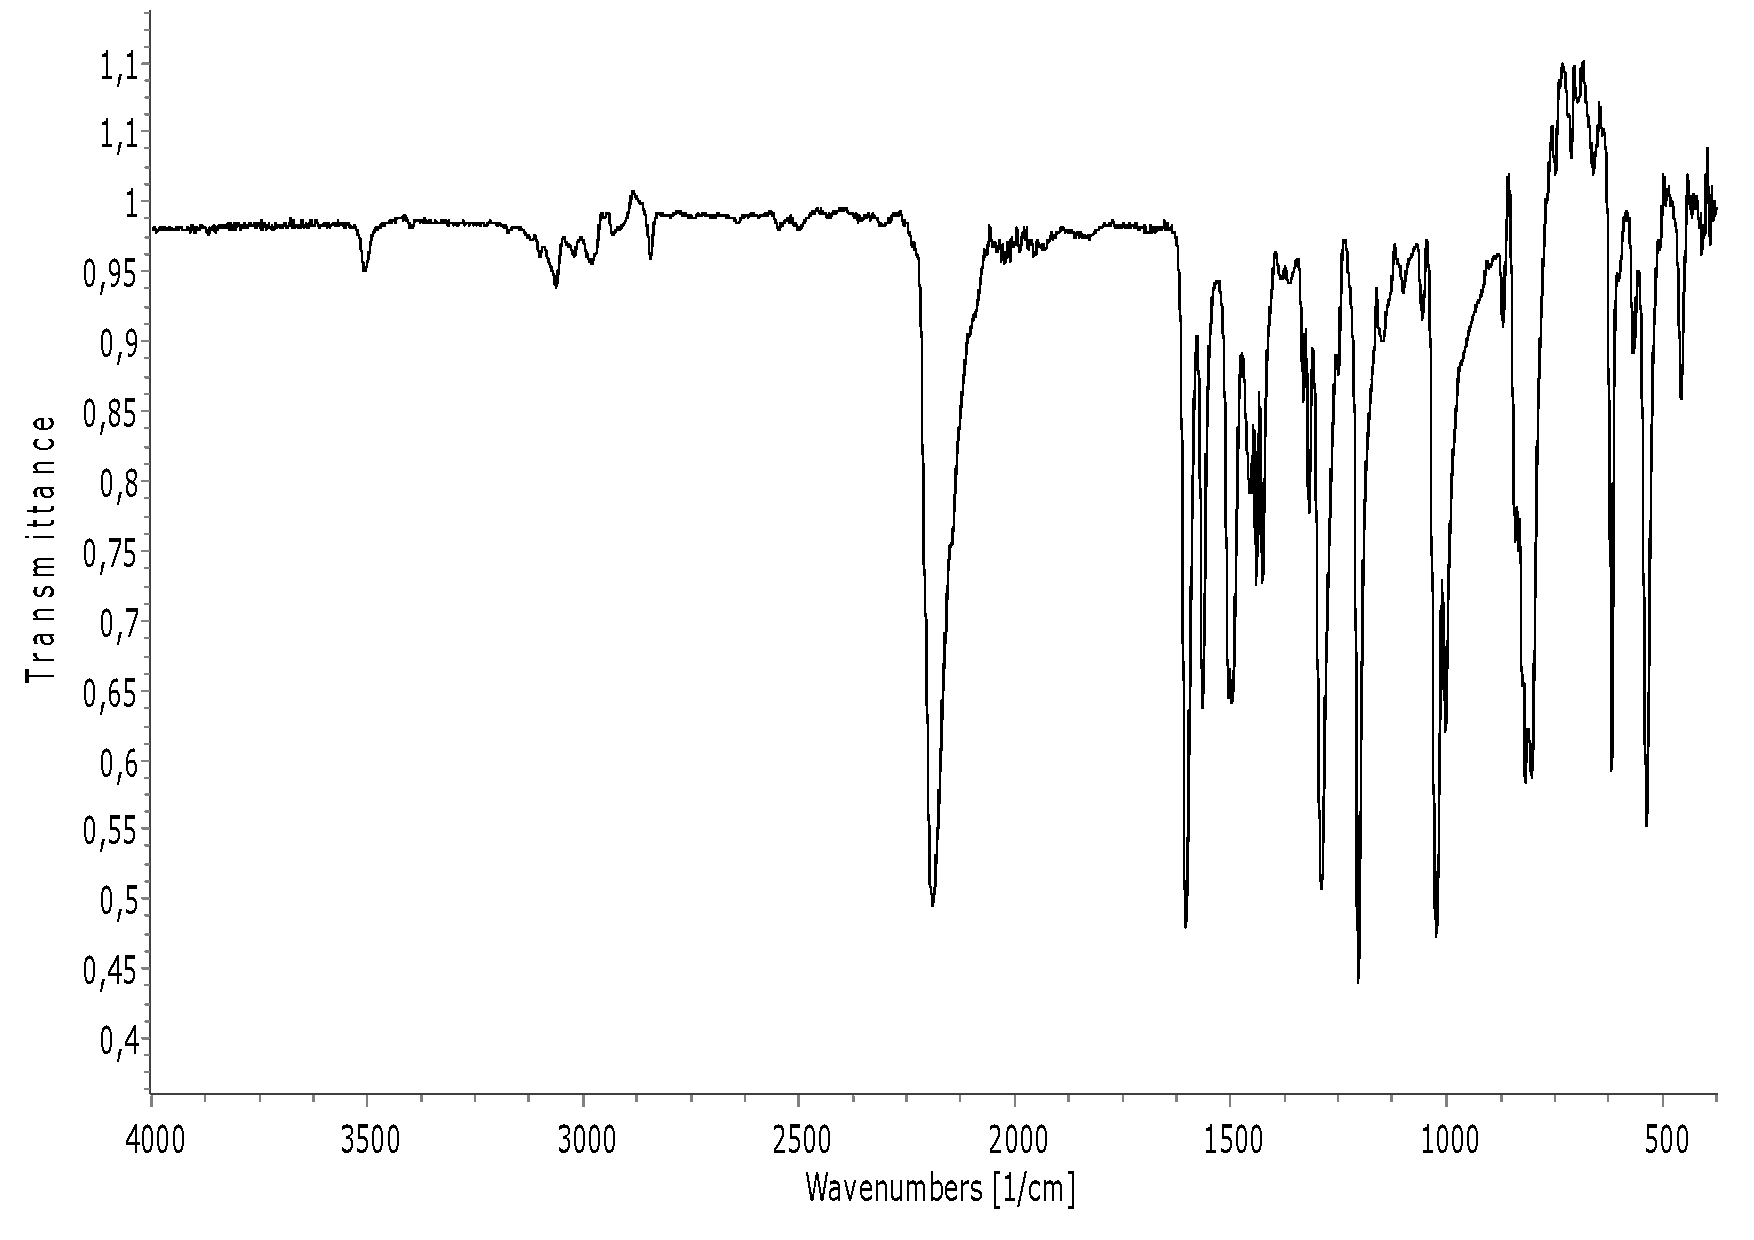
\includegraphics[width=1\textwidth]{figures/CoO4MOP-IR.pdf}
\caption{IR spectrum of \ce{[Co(OCN)_2(4-MeOpy)_4]}}
\end{figure}




\subsection{Structural characterization}
The crystal structure of \ce{[Co(OCN)_2(4-MeOpy)_4]} (perspective view is shown in fig. \ref{fig:CoO4MOP_pv}, a packing view in fig. \ref{fig:CoO4MOP_packv} and selected bond parameters are summarized in table \ref{batlb:CoO4MOP}) consists of two crystallographically independent mononuclear and neutral Co(II) complexes. Each Co(II) is six-coordinated by N atoms of two terminal cyanato anions, further by N donor atoms of four neutral 4-methoxypyridine molecules. The \ce{CoN_6} chromophores may be described as slighly distorted octahedra with trans-arrangement of the cyanato ligands. The Co-N bond lengths are in the range of 2.0601(16) to 2.2185(15) \AA, and the transoid N-Co-N bond angles within the \ce{CoN_6} octahedra vary from 176.19(6) to 179.04(6)$^\circ$. The bond parameters of the terminal cyanato anions are: Co-N-C: from 159.34(15) to 173.73(15)$^\circ$, N-C-O: from 178.5(2) to 179.5(2)$^\circ$, N-C: from 1.167(2) to 1.173(2) \AA, C-O: from 1.210(2) to 1.212(2) \AA.The shortest metal-metal separation is 8.5608(14) \AA. 


\begin{table}
\centering
\captionabove{Selected bond lengths (\AA) and angles ($^\circ$) for \ce{[Co(OCN)_2(4-MeOpy)_4]}}
\begin{tabular}{|l|l|l|l|}
\hline
Co(1)-N(1) & 2.0793(16) & Co(2)-N(7) & 2.0683(16)\\
\hline
Co(1)-N(2) & 2.0658(16) & Co(2)-N(8) & 2.0601(16)\\
\hline
Co(1)-N(3) & 2.1917(15) & Co(2)-N(9) & 2.2123(15)\\
\hline
Co(1)-N(4) & 2.1963(15) & Co(2)-N(10) & 2.1829(15)\\
\hline
Co(1)-N(5) & 2.2057(15) & Co(2)-N(11) & 2.1946(16)\\
\hline
Co(1)-N(6) & 2.2185(15) & Co(2)-N(12) & 2.1748(15)\\
\hline
N(1)-C(25) & 1.173(2) & C(25)-O(1) & 1.210(2)\\
\hline
N(2)-C(26) & 1.167(2) & C(26)-O(2) & 1.210(2)\\
\hline
N(7)-C(27) & 1.173(2) & C(27)-O(7) & 1.210(2)\\
\hline
N(8)-C(28) & 1.171(2) & C(28)-O(8) & 1.212(2)\\
\hline
\hline
N(1)-Co(1)-N(2) & 177.63(6) & N(7)-Co(2)-N(8) & 179.04(6)\\
\hline
N(5)-Co(1)-N(3) & 176.19(6) & N(10)-Co(2)-N(11) & 177.55(6)\\
\hline
N(6)-Co(1)-N(4) & 176.79(6) & N(9)-Co(2)-N(12) & 176.38(6)\\
\hline
Co(1)-N(1)-C(25) & 162.69(15) & N(1)-C(25)-O(1) & 179.04(17)\\
\hline
Co(1)-N(2)-C(26) & 173.73(15) & N(2)-C(26)-O(2) & 179.5(2)\\
\hline
Co(2)-N(7)-C(27) & 159.34(15) & N(7)-C(27)-O(7) & 178.55(19)\\
\hline
Co(2)-N(8)-N(28) & 161.66(15) & N(8)-C(28)-O(8) & 178.5(2)\\
\hline
\end{tabular}
\label{batlb:CoO4MOP}
\end{table}


\begin{figure}[!htpb]
\centering
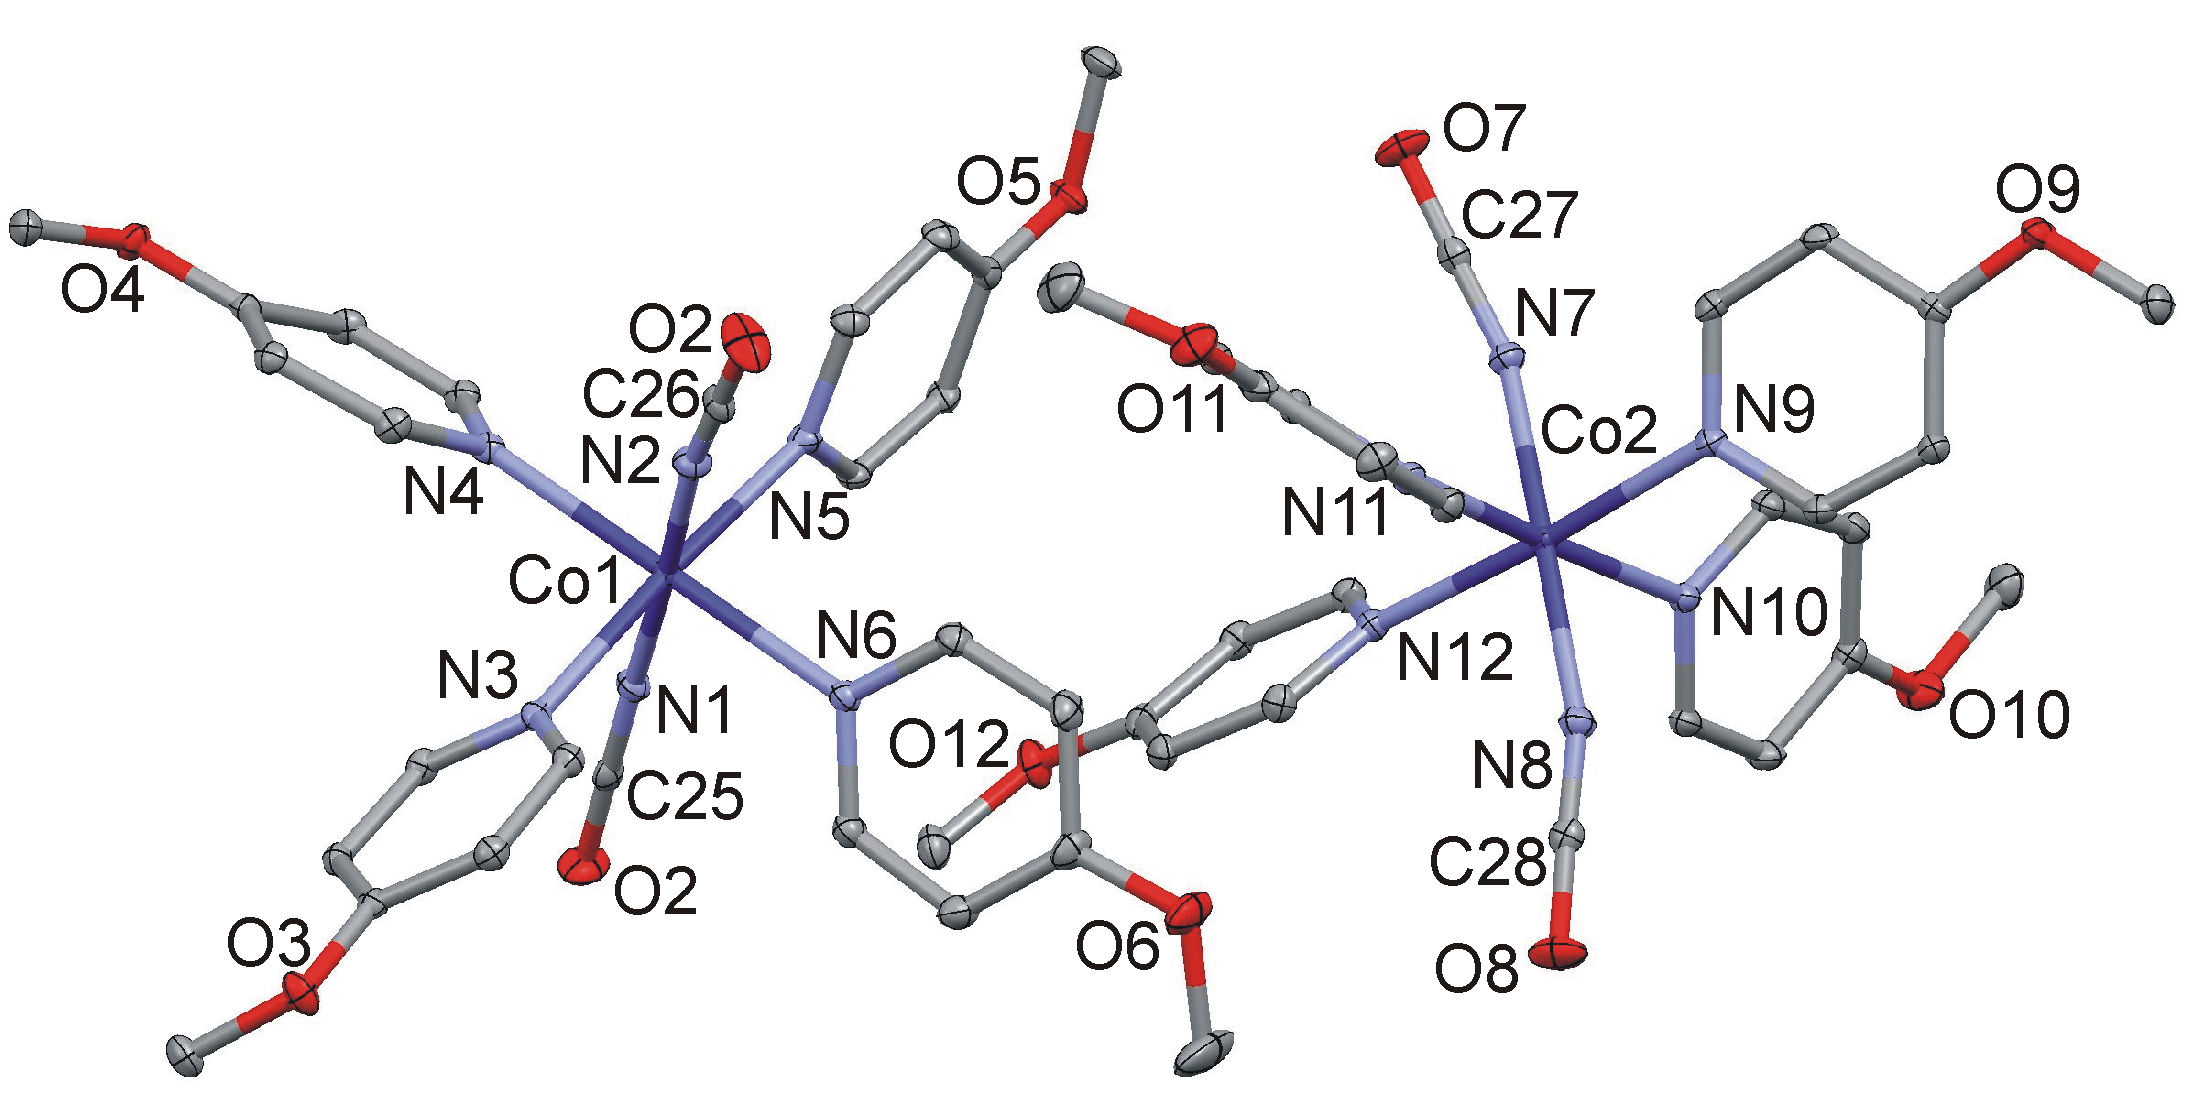
\includegraphics[width=1\textwidth]{figures/coomop_FIGm11.png}
\caption[Perspective view of \ce{[Co(OCN)_2(4-MeOpy)_4]}]{Perspective view of \ce{[Co(OCN)_2(4-MeOpy)_4]} with the atom numbering scheme.}
\label{fig:CoO4MOP_pv}
\vspace{\floatsep}
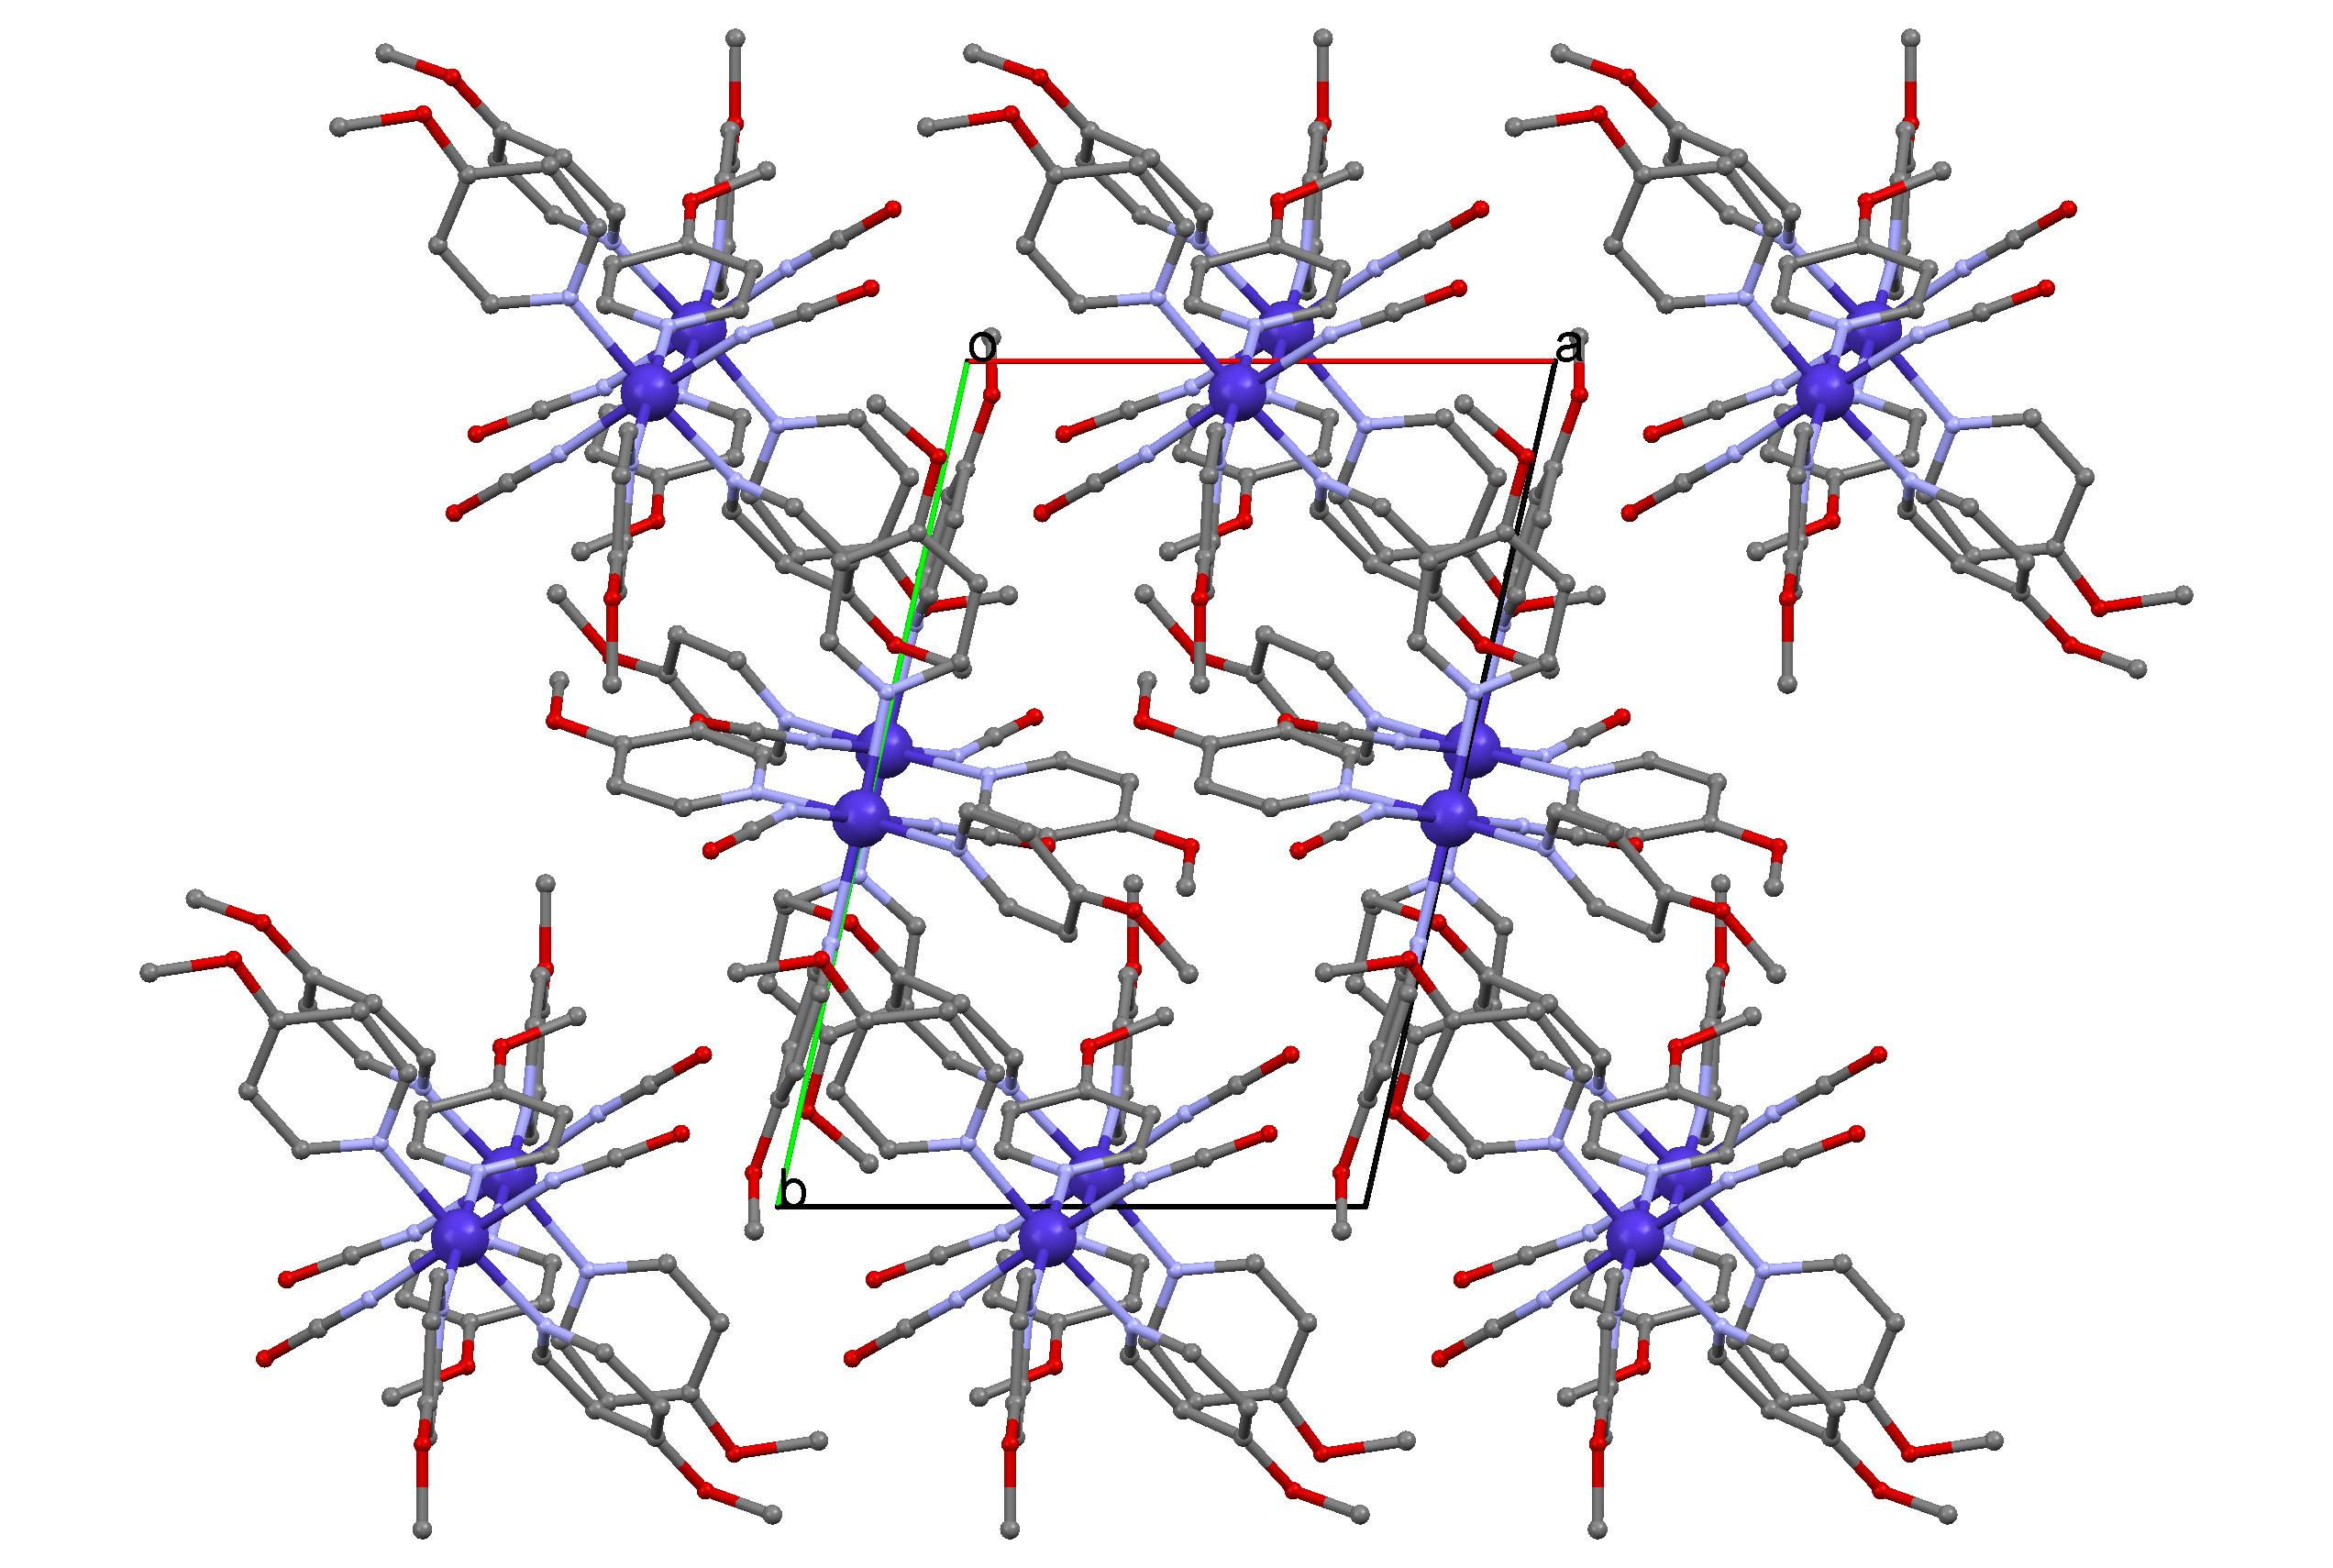
\includegraphics[width=1\textwidth]{figures/coomop_CC.png}
\caption{Packing view  of \ce{[Co(OCN)_2(4-MeOpy)_4]}.}
\label{fig:CoO4MOP_packv}
\end{figure}


\renewcommand{\arraystretch}{1.5}
\begin{table}
\centering
\captionabove{Crystallographic data and processing parameter of \ce{[Co(OCN)_2(4-MeOpy)_4]}}
\begin{tabular}{ | l |  l | }
\hline
Empirical formula & \ce{C_{26}H_{28}CoN_{6}O_{6}}\\
\hline
Formula mass & 579.47\\
\hline
System & triclinic\\
\hline
Space group & P-1\\
\hline
a ({\AA}) & 10.1989(12)\\
\hline
b ({\AA}) & 15.3641(18)\\
\hline
c ({\AA}) & 19.234(3)\\
\hline
$\alpha$ ($^\circ$) & 107.209(6)\\
\hline
$\beta$ ($^\circ$) & 102.632(7)\\
\hline
$\gamma$ ($^\circ$) & 98.012(5)\\
\hline
V (\AA$^{3}) $  & 2741.1(6)\\
\hline
Z & 4\\
\hline
T (K) & 100(2)\\
\hline
$\mu$ (mm$^{-1}$) & 0.677\\
\hline
 D$_{calc}$ (Mg/m$^{3}$) & 1.404\\
\hline
Crystal size (mm) & 0.23 x 0.18 x 0.12\\
\hline
$\theta$ max ($^\circ$) & 28.00\\
\hline
Data collected & 168102\\
\hline
Unique refl./ R$_{int}$ & 13238 / 0.0843\\
\hline
Parameters & 711\\
\hline
Goodness-of-Fit on F$^{2}$ & 0.994\\
\hline
R1 / wR2 (all data) & 0.0374 /0.0808\\
\hline
Residual extrema (e/\AA$^{3}$) & 0.35 /-1.49\\
\hline
\end{tabular}

\label{ptbl:CoO4MOP}

\end{table}

